我们将通过三个步骤定义可测函数的积分。首先定义非负简单函数的积分。以下设 $E$ 是 $\mathcal{R}^n$ 中的可测集。

\begin{definition}[可积性]
设 $ f(x)=\sum\limits_{i=1}^{k} a_i \chi_{A_i}(x)$ 是 $E$ 上的非负简单函数,其中 $\{A_1,A_2,\ldots$, $A_k\}$ 是 $E$ 上的一个可测分割,$a_1,a_2,\ldots,a_k$ 是非负实数。定义 $f$ 在 $E$ 上的积分为 1. 3
\begin{equation}
   \label{inter}
   \int_{E} f dx = \sum_{i=1}^k a_i m(A_i).
\end{equation}
一般情况下 $0 \leq \int_{E} f dx \leq \infty$。若 $\int_{E} f dx < \infty$,则称 $f$ 在 $E$ 上可积。
\end{definition}

一个自然的问题是,Lebesgue 积分与我们所熟悉的 Riemann 积分有什么联系和区别?之后我们将详细讨论 Riemann 积分与 Lebesgue 积分的关系。这里只看一个简单的例子。设 $D(x)$ 是区间 $[0,1]$ 上的 Dirichlet 函数。即 $D(x)=\chi_{Q_0}(x)$,其中 $Q_0$ 表示 $[0,1]$ 中的有理数的全体。根据非负简单函数积分的定义,$D(x)$ 在 $[0,1]$ 上的 Lebesgue 积分为
\begin{equation}\label{inter2}
  \int_0^1 D(x)dx = \int_0^1 \chi_{Q_0} (x) dx = m(Q_0) = 0
\end{equation}
即 $D(x)$ 在 $[0,1]$ 上是 Lebesgue 可积的并且积分值为零。但 $D(x)$ 在 $[0,1]$ 上不是 Riemann 可积的。

\begin{table}[htbp]
  \centering
  \small
  \caption{燃油效率与汽车价格}
    \begin{tabular}{lcc}
    \toprule
                  &       (1)         &        (2)      \\
    \midrule
    燃油效率      &   -238.90***      &      -49.51     \\
                  &    (53.08)        &      (86.16)    \\
    汽车重量      &                   &        1.75***  \\
                  &                   &       (0.641)   \\
    常数项        &  11253.00***      &    1946.00      \\
                  &  (1171.00)        &   (3597.00)     \\
    观测数        &     74            &      74         \\
    $R^2$         &      0.220        &       0.293     \\
    \bottomrule
    \end{tabular}%
  \label{tab:reg}%
\end{table}%

\begin{theorem}[Fubini 定理]\label{thm:fubi}
若 $f(x,y)$ 是 $\mathcal{R}^p\times\mathcal{R}^q$ 上的非负可测函数,则对几乎处处的 $x\in \mathcal{R}^p$,$f(x,y)$ 作为 $y$ 的函数是 $\mathcal{R}^q$ 上的非负可测函数,$g(x)=\int_{\mathcal{R}^q}f(x,y) dy$ 是 $\mathcal{R}^p$ 上的非负可测函数。并且
\begin{equation}\label{eq:461}
  \int_{\mathcal{R}^p\times\mathcal{R}^q} f(x,y) dxdy=\int_{\mathcal{R}^p}\left(\int_{\mathcal{R}^q}f(x,y)dy\right)dx.
\end{equation}
\end{theorem}

\begin{proof}
Let $z$ be some element of $xH \cap yH$.  Then $z = xa$ for some $a \in H$, and $z = yb$ for some $b \in H$. If $h$ is any element of $H$ then $ah \in H$ and $a^{-1}h \in H$, since $H$ is a subgroup of $G$. But $zh = x(ah)$ and $xh = z(a^{-1}h)$ for all $h \in H$. Therefore $zH \subset xH$ and $xH \subset zH$, and thus $xH = zH$.  Similarly $yH = zH$, and thus $xH = yH$, as required.
\end{proof}

回归分析 (regression analysis) 是确定两种或两种以上变量间相互依赖的定量关系的一种统计分析方法。根据定理~\ref{thm:fubi},其运用十分广泛,回归分析按照涉及的变量的多少,分为一元回归和多元回归分析;按照因变量的多少,可分为简单回归分析和多重回归分析;按照自变量和因变量之间的关系类型,可分为线性回归分析和非线性回归分析。

\begin{figure}[htbp]
  \centering
  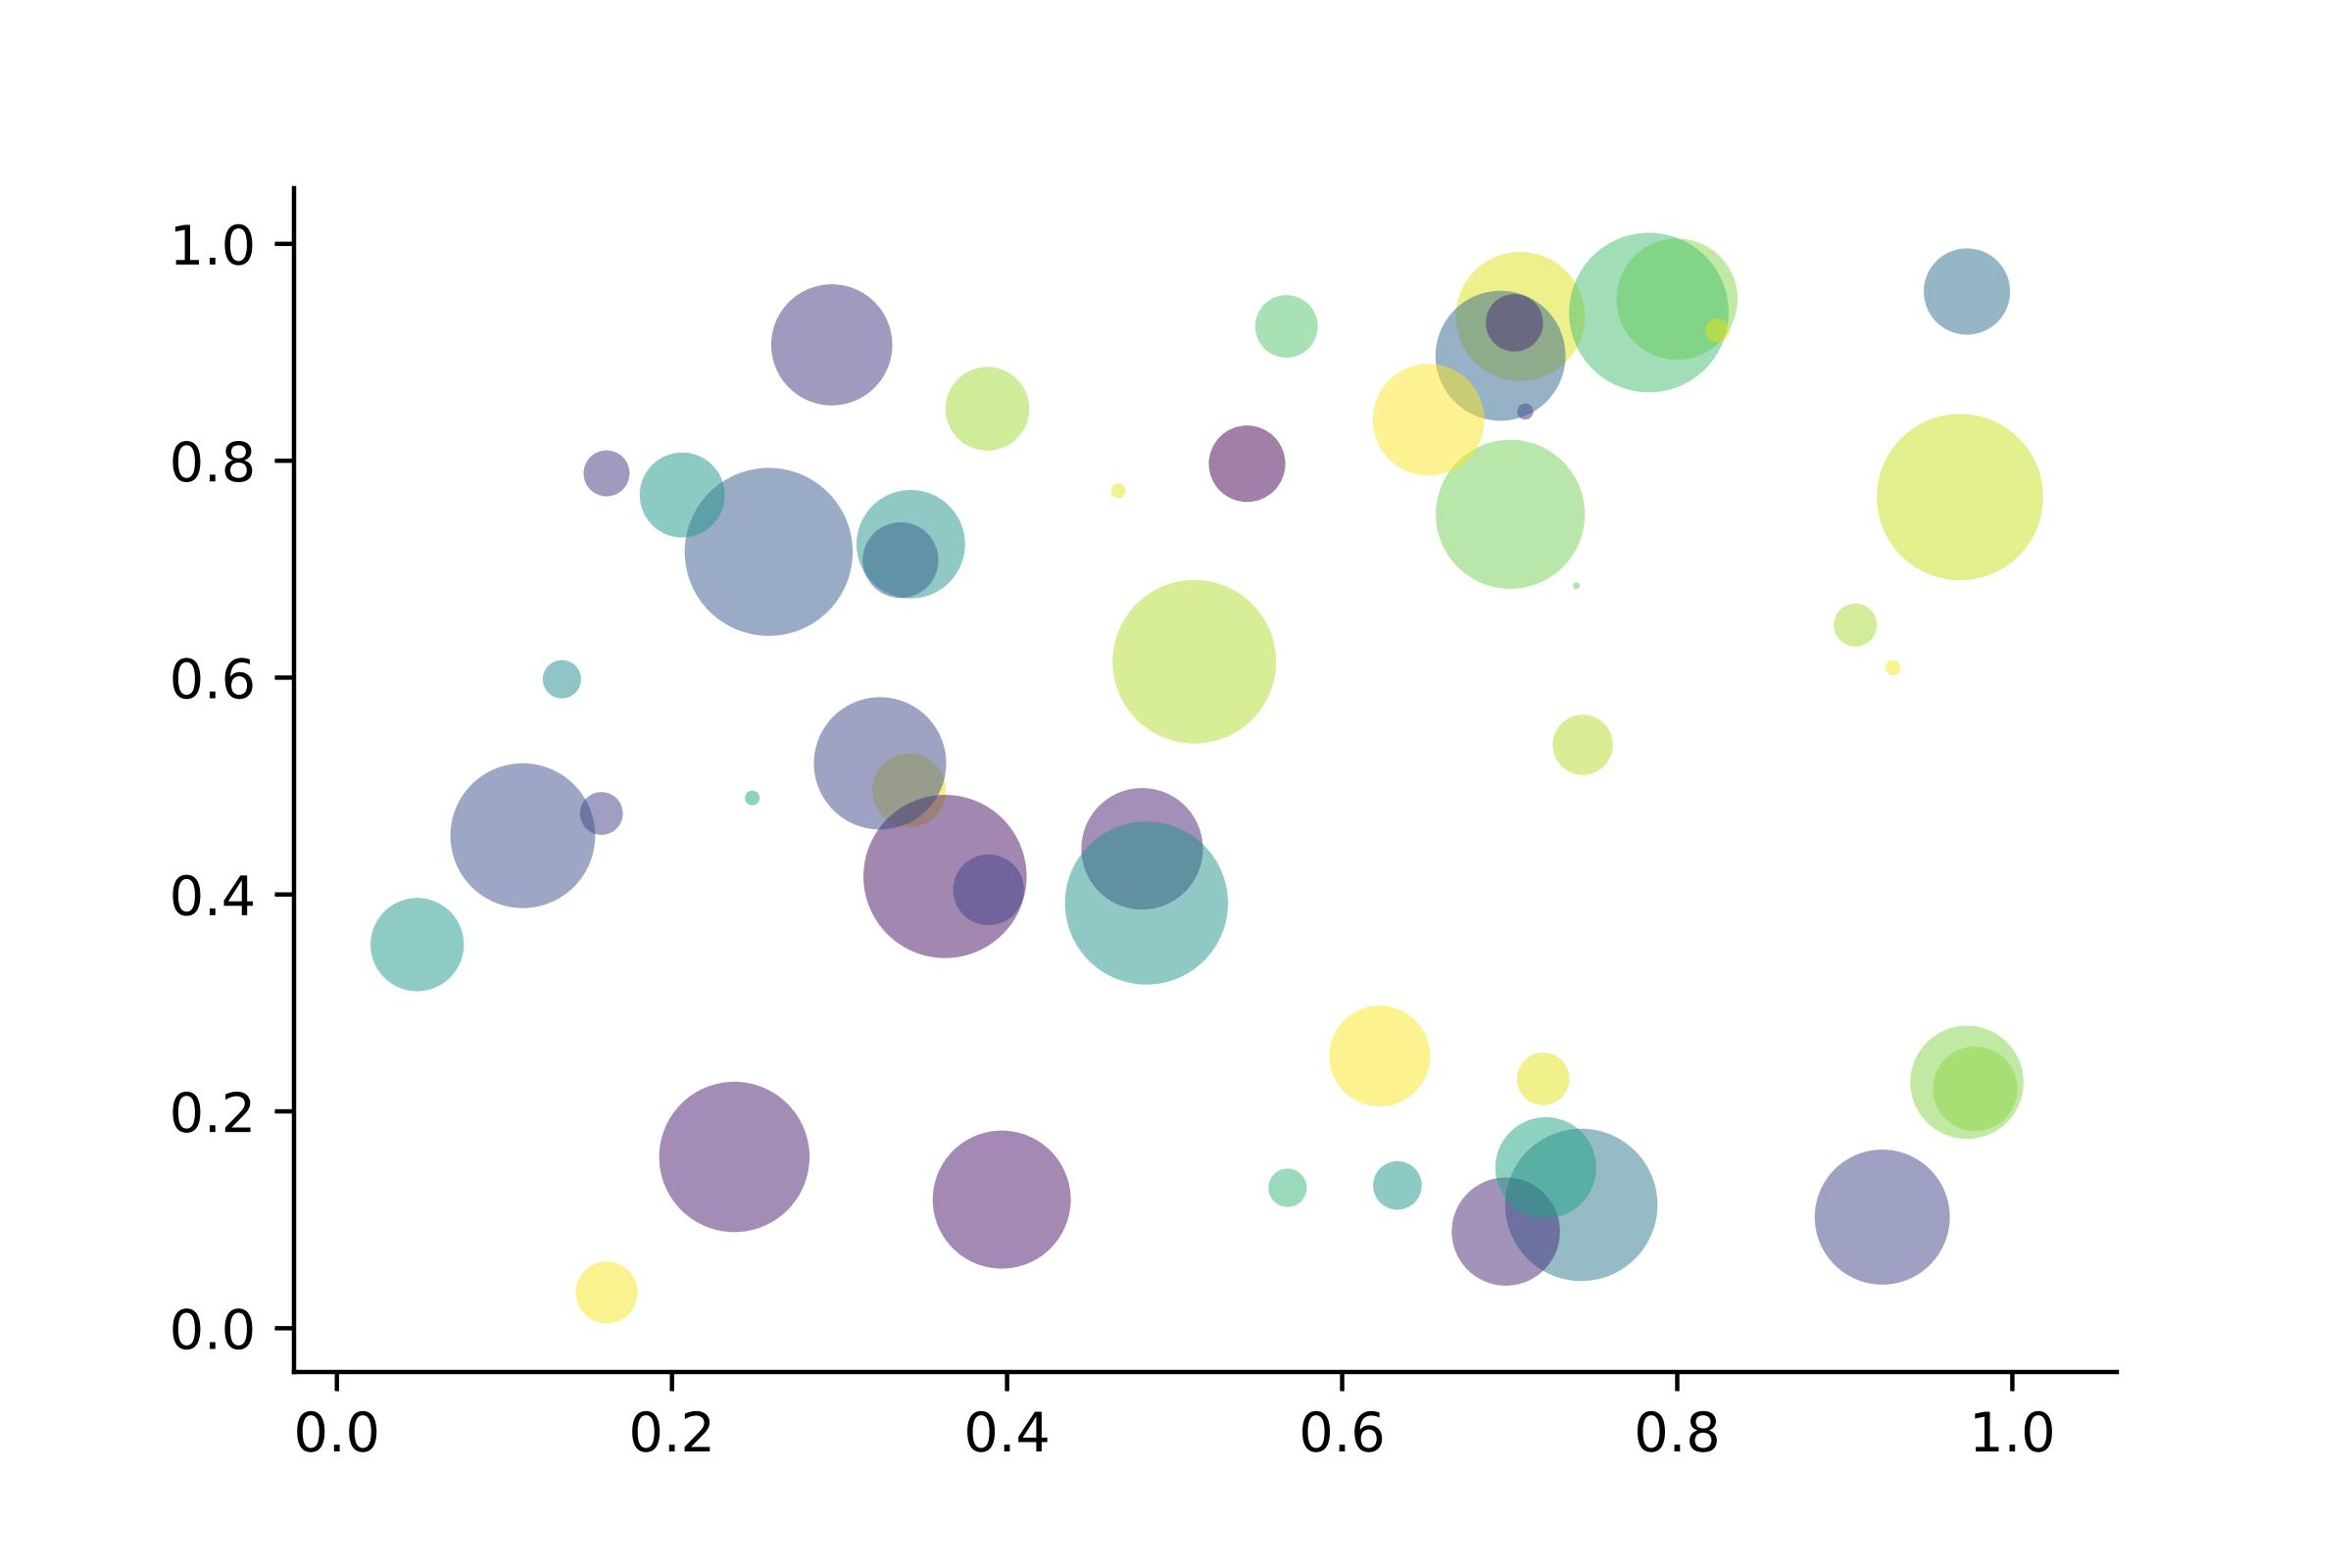
\includegraphics[width=0.5\textwidth]{scatter.jpg}
  \caption{散点图示例 $\hat{y}=a+bx$ \label{fig:scatter}}
\end{figure}